\documentclass[../thesis.tex]{subfiles}
\begin{document}

%% Intro to RL
Reinforcement learning (RL) provides a mathematical formalism for learning-based control. Specifically, reinforcement learning techniques can automatically discover and acquire near-optimal behavior (often referred to as policies), which optimizes a user-specified reward function. The reward function defines \emph{what} a policy should do, and an RL algorithm automatically determines \emph{how} to do it. Devising RL algorithms has been an active area of research ever since the development of dynamic programming algorithms for optimal control in the 1960s~\citep{bellman1966dynamic}. Over the last decade, the introduction of effective high-capacity deep neural network function approximators into RL, along with effective algorithms for training them, has allowed RL methods to attain excellent results along a wide range of domains~\citep{tesauro1994td,levine2013guided,mnih2013playing,levine2016end,silver2017mastering,kalashnikov2018qtopt}, often producing policies that match or outperform the best known control strategy for the downstream task. 

% Interaction is impractical
Despite these promising results, reinforcement learning methods have had limited applicability in a number of other decision-making and control problems in the real world. This is because traditional reinforcement learning techniques that have been developed for a few decades now typically subscribe to an \emph{online} learning paradigm: these techniques involve iteratively collecting experience by actively interacting with an environment in a trial-and-error fashion, and then using that experience to improve the policy~\citep{sb-irl-98}. In many settings, this sort of online interaction is impractical, either because data collection is expensive (e.g., in robotics, drug design, education, power grid management, or healthcare) and dangerous (e.g., in autonomous driving, power grid management, or healthcare). One option to circumvent the need for active interaction is to instead build simulators for the target problem and then run RL in simulation for discovering the optimal behaviors. Even though this approach is practically feasible, it tends to perform poorly when accurate simulators are hard to build (e.g., modelling the interaction between a drug and a pathogen or that between humans and robots).

% Motivate dataset-driven
An alternate approach that we take in this dissertation is to \textbf{build a ``dataset-driven'' paradigm for RL that can incorporate static, previously-collected datasets for making effective decisions}. Since the success of supervised and unsupervised machine learning methods across a range of practically relevant problems over the past decade can in large part be attributed to the development of scalable dataset-driven learning methods, which continue to reliably improve as they are trained with more and higher-quality data, one would also expect that such a dataset-driven paradigm for RL will enjoy these appealing properties. Put in other words, such a dataset-driven paradigm for RL bears the promise of translating progress in collecting datasets and advances in deep learning, directly to generalizable and powerful decision-making engines. 

\begin{wrapfigure}{r}{0.4\textwidth} 
    \vspace{-10pt}
    \centering
    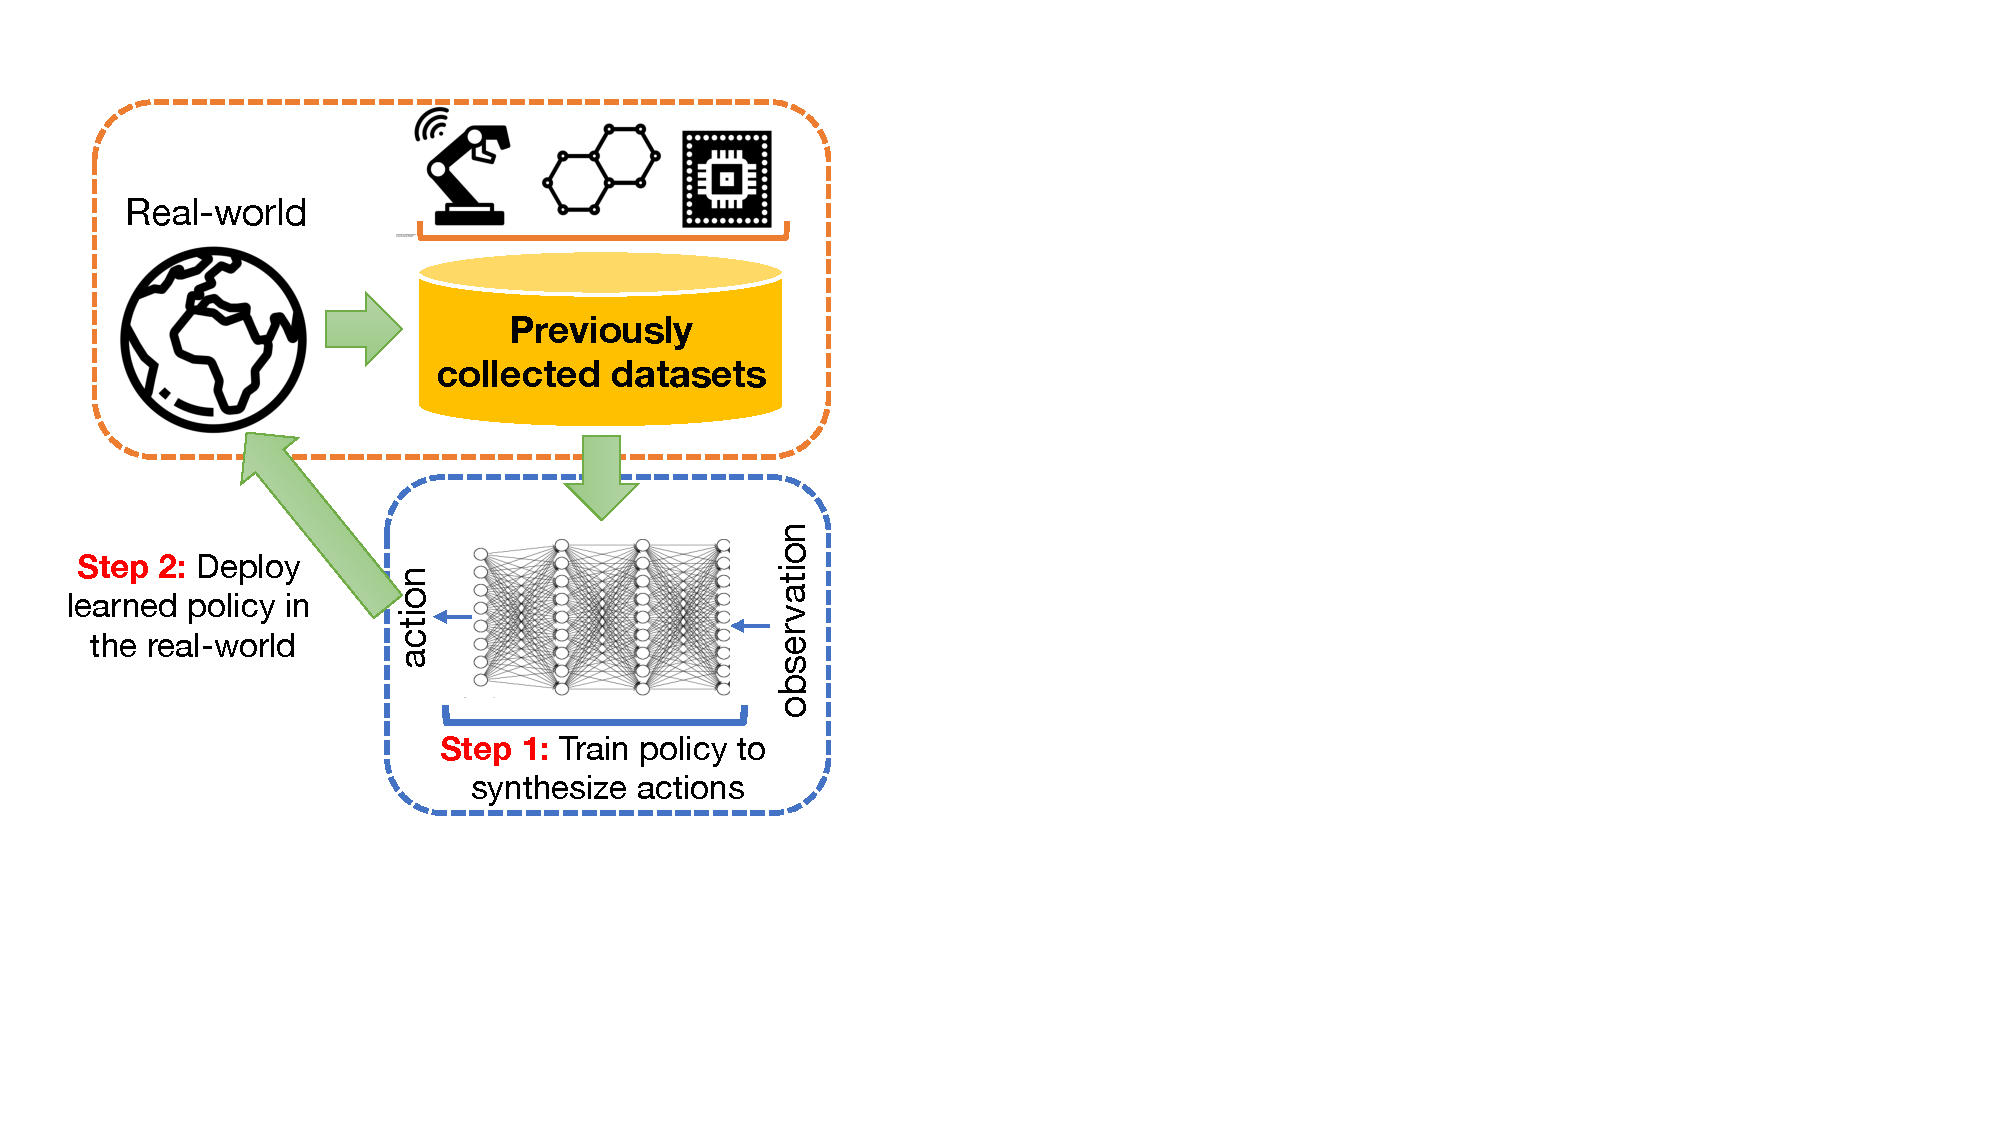
\includegraphics[width=0.99\linewidth]{offline_rl_fig.pdf}
    \vspace{-0.5cm}
    \caption{\label{fig:offline_rl_sketch} \footnotesize{The offline RL paradigm.}}
    \vspace{-0.5cm}
\end{wrapfigure}
% Why instantiating this is hard
That said, instantiating this paradigm presents a challenge as it requires reconciling the \textbf{passive} nature of a static dataset with traditional RL techniques and objective functions, which critically rely on \textbf{actively} collecting experience for improving the underlying policy. While prior work shows that the class of off-policy RL algorithms, which we briefly review in Chapter~\ref{chapter:problem_statement}, can suffice for this fully offline setting as well~\citep{lange2012batch,chen2019information,munos2003errorapi,munos2005erroravi}, these classical techniques often require restrictive assumptions that do not hold with high-dimensional control problems and realistic datasets. As we will discuss in Chapter~\ref{chapter:diagnosing}, in realistic decision-making problems, the inability to actively collect experience often manifests in the form of several challenges pertaining to distributional shift, generalization, and optimization. These challenges are perhaps the most evident in the fully \emph{``offline''} setting, where we are not allowed access to any form of active interaction. Function approximators such as deep neural networks generally exacerbate these issues, since function approximation increases the vulnerability of the learning algorithm to pathologies from distributional shift and incorrect generalization.

% what we do
Concretely, in this dissertation we provide a theoretical and empirical foundation to the problem of utilizing static datasets in reinforcement learning, especially relevant within the context of realistic datasets. We perform empirical studies to isolate the various challenges when learning policies via RL in a fully offline manner, followed by developing algorithmic techniques to address these challenges. Then, we develop techniques to scale up these algorithmic ideas to leverage the generalization benefits offered by highly-expressive function approximators, especially when provided with diverse and multi-task datasets from a rich set of RL problems. We also develop techniques that enable rapid fine-tuning of an offline initialization learned from the static dataset, with a limited amount of active interaction. Finally, we demonstrate the efficacy of these algorithmic ideas in the context of two real-world decision-making problems in hardware accelerator design (i.e., chip design) and real robot control.  

% However, the appeal of a fully offline reinforcement learning framework is enormous: in the same way that supervised machine learning methods have enabled data to be turned into generalizable and powerful \emph{pattern recognizers} (e.g., image classifiers, speech recognition engines, etc.), offline reinforcement learning methods equipped with powerful function approximation may enable data to be turned into generalizable and powerful \emph{decision making engines}, effectively allowing anyone with a large enough dataset to turn this dataset into a policy that can optimize a desired utility criterion. From healthcare decision-making support to autonomous driving to robotics, the implications of a reliable and effective offline reinforcement learning method would be immense.


% A ``dataset-driven'' paradigm broadens the applicability of RL to a variety of decision-making problems where historical datasets already exist or can be collected via domain-specific strategies. It also brings the scalability and reliability benefits that modern supervised and unsupervised ML methods enjoy into RL. 
% That said, instantiating this paradigm is challenging as it requires reconciling the \textbf{static} nature of the dataset with RL, that critically rely on \textbf{dynamically} answering counterfactual queries for learning.
% That said, instantiating this paradigm is fundamentally challenging as we must reconcile the \textbf{static} nature of learning from a fixed dataset with the \textbf{dynamic} and \textbf{active} nature of traditional RL methods. 
% My work shows that this distinction often manifests in the form of challenges pertaining to distribution shift, generalization and optimization. As a result, we need to develop new RL approaches for leveraging static datasets. 

% Indeed,  While this was arguably less of an issue when reinforcement learning methods utilized low-dimensional or linear parameterizations, and therefore relied on small datasets for small problems that were easy to collect or simulate~\citep{lange2012batch}, once deep networks are incorporated into reinforcement learning, it is tempting to consider whether the same kind of data-driven learning can be applied with reinforcement learning objectives, thus resulting in \emph{data-driven reinforcement learning} that utilizes only previously collected offline data, without any additional online interaction~\citep{kumar_blog,d4rl}. See Figure~\ref{fig:introduction} for a pictorial illustration. A number of recent works have illustrated the power of such an approach in enabling data-driven learning of policies for dialogue~\citep{jaques2019way}, robotic manipulation behaviors~\citep{ebert2018visual,kalashnikov2018qtopt}, and robotic navigation skills~\citep{kahn2020badgr}.

\textbf{Organization.} After a brief disscussion of notation and the problem statement in Chapter~\ref{chapter:problem_statement} (based on \citet{levine2020offline}), we make the following contributions:  
\begin{itemize}
    \item In Chapter~\ref{chapter:diagnosing}, we empirically analyze the behavior of traditional RL algorithms in the offline learning setting and isolate the challenges of distributional shift and overfitting. This work appeared previously as \citet{fu2019diagnosing}.
    \item In Chapter~\ref{chapter:bear}, we develop an initial algorithm to circumvent the challenge of distributional shift by restricting the learned policy to lie within the \emph{support} of the data-collection policy. This work was published previously as \citet{kumar2019stabilizing}.    
    \item In Chapter~\ref{chapter:cql}, we develop an approach for learning policies from static data, that we call conservative value estimation. Conservative estimation of value functions dispenses with the need to restrict the learned policy to within the support of the data-collection policy, enabling bigger performance improvements, while still addressing the challenge of distributional shift. We also instantiate our approach into concrete model-free and model-based algorithms. This chapter consists of content from work previously published as \citet{kumar2020conservative,yu2021combo}.
    \item In Chapter~\ref{chapter:scaling}, we develop explicit regularization techniques that enable the approach from Chapter~\ref{chapter:cql} to utilize high-capacity neural network architectures. This chapter is based on works previously published as \citet{kumar2021dr3,kumar2023offline}.
    \item In Chapter~\ref{chapter:cds_uds}, we develop automatic data sharing and reward labeling strategies that boost the performance of the approach from Chapter~\ref{chapter:cql}, when learning from multi-task and unlabeled datasets. This chapter consists of work that was published as \citet{yu2021conservative,yu2022leverage}.
    \item In Chapter~\ref{chapter:calql}, we develop a method that enables sample-efficient online fine-tuning of offline policy initializations learned by the approach in Chapter~\ref{chapter:cql}. This chapter is primarily based on work that previously appears as \citet{nakamoto2023calql}.
    \item In Chapter~\ref{chapter:ptr}, we present an application of the techniques from Chapters~\ref{chapter:cql}, \ref{chapter:scaling}, and \ref{chapter:calql} to the problem of incorporating broad prior data for boosting generalization of robotic skill learning, with only a handful of task-specific rollouts. This chapter consists of work that was previously published as \citet{kumar2022pre}.
    \item In Chapter~\ref{chapter:prime}, we present an application of the techniques from Chapter~\ref{chapter:cql} to the problem of hardware accelerator design. This chapter consists of work that was published as \citet{kumar2021data}.       
\end{itemize} 

We conclude with a discussion of current approaches and promising future directions in developing reinforcement learning algorithms that can incorporate static datasets.

%  With the advent of deep neural networks and their immense power in modelling visual data, the focus has recently shifted to modelling monocular cues implicitly with a CNN and predicting 3D from a single image as depth/surface orientation maps or 3D voxel grids.

% Talk about 3D reconstruction. How it has been approached traditionally. Brief history of 3D reconstruction. From blocks world to sfm to mvs. Mention faces as a special case of an object category. Talk about faces as a well studied object category. blanz and vetter. kemelmacher-schlizerman etc. Been traditionally hard for generic object categories due to greater variation in shapes etc.

% Recognition systems have improved leaps and bounds in recent times. We can detect objects in images, segment out the pixels for objects etc. Such outputs provide essential cues to 3D perception as well. For example, the silhouette provides information about the 3D shape. The relative locations of keypoints in a 2D image inform the global 3D pose of the object. 

% Gaps in literature: models for complex objects, low shot object reconstruction, a stable framework for integrating semantic reasoning into reconstruction.
% Contributions of this thesis:
% Use statistical machine learning techniques to reason about 3D perception cues from diverse image collections. Using recognition systems in the loop for informing object reconstruction. Adapting 
% \begin{itemize}
% \item Building statistical models for 3D shapes for diverse object categories beyond faces and using them in conjunction with recognition techniques for fully automatic single-view 3D reconstruction.
% \item Enriching the output of object detection systems with real world heights of objects by predicting their amodal extent in scenes.
% \item Unifying single and multi-view 3D object reconstruction by incorporating geometric constraints in state-of-the-art recognition systems (CNNs)
% \end{itemize} 

% Brief summary of the thesis. In chapter 2, we talk about our system to learn category specific deformable 3D models..... In chapter 3, we presnet amodal.... Finally in chapter 4, we present LSMs, where we learn in a data driven manner with CNNs while incorporating epipolar geometry constraints. 
\end{document}